\documentclass[main.tex]{subfiles} 

\begin{document}

\section*{Undervisningsopplegget}
\label{sec:1}
Fokuset i undervisningen jeg vil utføre i 8. klassen vil være rundt begrepene celler og celledeling. 
I tillegg skal elevene instrueres i å skrive en rapport til et eksperiment de skal utføre i laboratoriet.
Hensikten med opplegget er å formidle til elever vanskelige begreper fra naturfag slik at de kan lettere 
se sammenhenger mellom temaer. Temaer som forøvrig blir memorisert og forstått i henhold til nivåene 
som er definert utfra kompetansemålene. 

Undervisningen er fordelt på 3 skoletimer over 2 uker. Opplegget utførte jeg alene, med veileder og en 
medstudent som observatører. De bidro også i blant med å gi veiledning når elevene jobbet enten 
selvstendig eller sammen i grupper. De første to timene forekommer i klasserommet, mens den siste timen 
i laboratoriet.

\subsection*{1. time}

Hensikten med denne timen er å oppsummere det elevene har lært hittil om celler og 
levende organismer, og innføre et nytt tema om encellede organismer. Timen starter med repetisjon 
av det elevene har lært fra tidligere timer, deriblant om mikroskop og cellestrukturen. Ved oppstart 
av timen initieres elevene til å reflektere over temaer og begreper de har lært og hatt lekser 
om.
 
Siden elevene gjennom helklassesamtalen har blitt "varmet" opp kognitivt, er de mottagelige for å 
lære om et nytt tema. Innføringen av nytt tema er bevisst satt opp på en slik måte at overgangen 
fra repetisjon til det nye temaet blir naturlig og flytende. Dette vil bidra til å la elevene danne et 
helhetlig bilde om celler. I timene hvor de har hatt en innføring om celler, har de lært om basale 
strukturer. I denne timen går de litt dypere ved å få en innføring om en av klassifikasjonene av celler.
Hensikten med innføringen er todelt : å gjøre elevene bevisst om at det finnes forskjellige type
celler, og forberede de for den siste timen hvor de vil studere slike celler under mikroskop.
 
I den siste øvelsen skal elevene jobbe sammen med tokolonnenotatet i grupper (se 
vedlegg \ref{sec:tokolonnenotat}), hvor de blir enige med hverandre om hva som er viktig å formidle videre 
om deres felles temaer. Deretter fordeles de i nye grupper slik at hver gruppe har minst en elev som har 
forbredt sitt sett med begreper. Under hele denne prosessen er vi tilgjengelige og går rundt for å 
høre elevene diskutere begreper, først sammen i grupper, og deretter individuelt når de fremfører sine 
konklusjoner med medelever. Hvis vi observerer at eleven har problemer med å gi tilstrekkelig 
respons på et gitt tema, initierer vi eleven i en dialog hvor vi forsøker å sammen konstruere en 
mer utdypet forståelse av begrepene. 

\subsection*{2. time}

Til denne timen bruker jeg navnekort, hvor en elevs navn blir opplest vilkårlig fra en usortert liste, 
og deretter får eleven 
ordet og tid til å respondere. Elevrespons blir enten akseptert, eller hvis eleven viser svakheter
i sin forståelse blir spørsmålet gitt til andre i klassen. Dialogen blir avsluttet med en vurdering,
og hvis nødvendig blir tilleggsinformasjon supplert. 

\begin{figure}[h!]
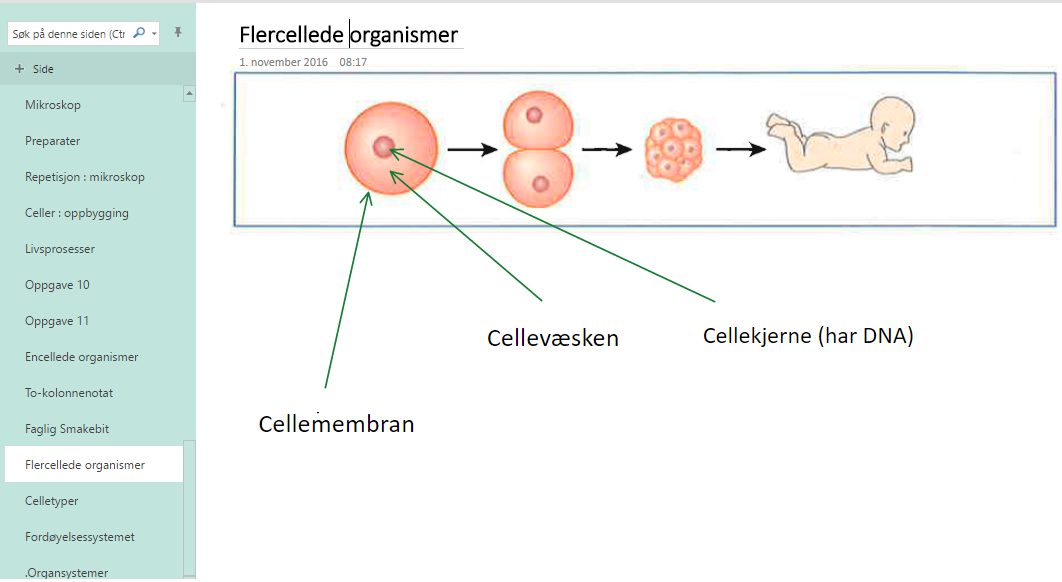
\includegraphics[scale = 0.6]{../figures/onenote_flercellet.png}
\caption{notat 1}
\label{fig:notat1}
\end{figure}

Opplegget er laget hensiktsmessig for å forsterke forståelsen for begrepet flercellet organisme og dens utvikling fra 
en enkelt celle (se figur \ref{fig:notat1}). For å få til dette starter timen med temaet encellede organismer, 
videre til skillet mellom forskjellige typer celler og hvordan de er med å danne vev, og prosessen fra vev til
organer, og fra organer til organssystemer. Når organsystemer blir introdusert benyttes 
en anatomisk modell av overkroppen. Den brukes til å snakke om fordøyelsessystemet.
Den anatomiske modellen består av organer som er avtagbare (nesten som legoklosser) og flere organer 
som ligger i bakgrunnen kan dermed ses. Gjennom hele forklaringen om fordøyelsessystemet brukes
elevene underveis ved hjelp av kontrollspørsmål. De bidrar med å gi en forklaring for hele prosessen, 
fra maten blir tygd til den blir brutt ned i tarmene og næringen blir tatt opp gjennom blodstrømmen, 
og tilslutt avfall som blir utskilt fra endetarmen. Prosessen gjentas på OneNote (se figur \ref{fig:notat2}). 
Etter at alle temaene har blitt gjennomgått, begynner den samme prosessen, 
men med omvendt rekkefølge, med hensikten å vise at mennesker består av milliarder av celler og 
at vi kan spore vår oppvekst tilbake til befruktningsprosessen, hvor vårt opphav er nemlig som
encellede organismer. Ved å bruke denne fremgangsmåten merket jeg at konseptene ble grundigere
gjennomgått og rekkefølgen virket logisk og oversiktelig. Gjentagelsen av prosessen i motsatt
rekkefølge ble brukt til å forsterke elevenes forståelse for begrepene og danne en logisk 
overgang i deres tankebaner. 

\begin{figure}[h!]
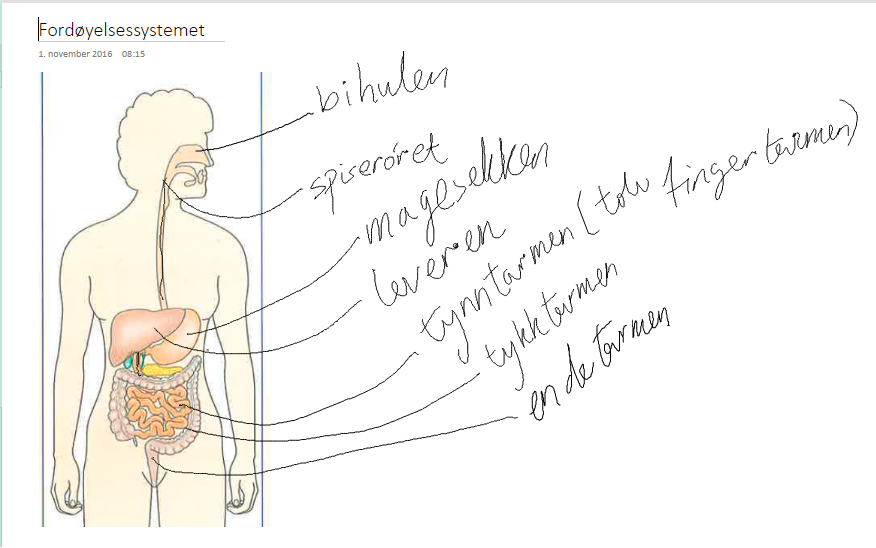
\includegraphics[scale = 0.6]{../figures/onenote_fordoyelse.png}
\caption{notat 2}
\label{fig:notat2}
\end{figure}

\subsection*{3. time}

Timen starter hvor jeg fører opp målet med timen på tavlen, noe jeg foreløpig ikke har gjort. Deretter 
informeres elevene om hvordan prøvene ble innsamlet
og hvordan de skal studeres under et mikroskop. Etter at informasjonen har blitt formidlet både
muntlig og skriftlig (på tavlen) bes elevene om å lese om øvelsen i læreboken. Deretter
fordeles de i grupper og elevene får utdelt roller i gruppene. Noen i gruppene henter
mikroskop og objetivglass, mens andre henter utstyr som dråpeteller, vannprøver og bomull.
Etter at elevene har samlet utstyr og er klare til å studere prøvene, informeres de
om hvordan de kan bruke bomull til å absorbere vannprøvene og studere organismene under mikroskopet.
Siden elevene har brukt mikroskopene fra en tidligere laboratorieøvelse, blir de bedt om å 
gjennomføre resten av forsøket på egenhånd. Etter at alle instruksene har blitt delt ut går vi
rundt og observerer elevene. 
En del av gruppene har problemmer med for eksempel overbruk av bomull, 
eller så tilsetter de for lite/mye vann på objektglasset. Noen av gruppene får hjelp med å finne 
riktig innstillinger for å studere organismene. 
Samtidig forbereder vi vår egen prøve i mikroskopet som er koblet til en datamaskin. Etter at alle elevgruppene 
har klart å observere mikroorganismene og deres oppførsel, utfører vi eksperimentet på vårt eget mikroskop.
Deretter instruerer vi elevene til å studere en annen prøve som var innsamlet fra en forskjellig kilde. Elevene 
gjentar forsøket og danner nye observasjoner. 
Tilslutt gjennomgåes hva de forskjellige gruppene observerte og elevene blir bedt om å lage en rapport som skal 
leveres inn på It's Learning. Siden dette var første gangen de har blitt bedt om å lage en rapport i naturfagstimen, 
informeres elevene om hva som forventes skal stå i rapporten.

\end{document}